\chapter{SatNOGS: Глобальная сеть наземных спутниковых станций с открытым исходным кодом}

SatNOGS представляет собой комплексную платформу \cite{satnogs_general_docs},
обеспечивающую функционирование открытой сети наземных станций для мониторинга
спутников. Основной целью проекта является разработка полного стека открытых
технологий, основанных на открытых стандартах, и создание полноценной наземной
станции в качестве демонстрации возможностей данного стека.

Система SatNOGS способна принимать сигналы со спутников, находящихся на низкой
околоземной орбите (LEO), в диапазонах UHF и VHF. Она позволяет извлекать
сигналы состояния и телеметрии, данные с научных и исследовательских спутников
(например, результаты магнитосферных экспериментов), метеорологические данные и
другую информацию.

Проект SatNOGS включает в себя несколько ключевых компонентов: веб-приложение
для планирования наблюдений, базу данных для хранения информации о спутниках,
клиентское программное обеспечение для работы на наземных станциях и аппаратное
обеспечение с открытым исходным кодом. Все это создает модульную архитектуру,
позволяющую легко интегрировать новые функции и расширять функциональность
системы.

SatNOGS активно развивает сообщество пользователей и разработчиков, предлагая
доступ к документации и инструментам для создания собственных наземных станций.
Это создает возможности для участия в глобальной сети наблюдений за спутниками
и обмена данными между участниками проекта.

\section{Компоненты SatNOGS}

SatNOGS включает в себя несколько ключевых компонентов, каждый из которых играет
важную роль в функционировании платформы, см. рисунок~\ref{fig:satnogs_data_flow}.
Ниже представлена таблица \ref{tab:satnogs_components}, описывающая основные элементы системы:

\begin{table}[H]
	\caption{Основные компоненты системы SatNOGS}
	\centering
	\begin{tabular}{|l|p{10cm}|}
		\hline
		\textbf{Компонент}       & \textbf{Описание}                         \\
		\hline
		SatNOGS Network          & Веб-приложение, предназначенное для
		планирования наблюдений по сети наземных станций. Оно способствует
		координации наблюдений за спутниковыми сигналами и планированию таких
		наблюдений среди наземных станций, подключенных к сети.              \\
		\hline
		База данных SatNOGS      & Ресурс, позволяющий пользователям
		предоставлять информацию о передатчиках активных спутников. Данные
		доступны через API или веб-интерфейс.
		\\
		\hline
		Клиент SatNOGS           & Программное обеспечение, работающее на
		наземных станциях (обычно на встраиваемых системах). Оно получает
		регулярные задания на наблюдение из сети, принимает спутниковые передачи
		и отправляет их обратно в веб-приложение Network.                    \\
		\hline
		Наземная станция SatNOGS & Аппаратное обеспечение наземной станции с
		открытым исходным кодом, включающее ротаторы, антенны и электронику,
		подключенные к клиенту.
		\\
		\hline
		SatNOGS Dashboard        & Веб-интерфейс для визуализации и анализа
		данных телеметрии, полученных от спутников. Он предоставляет
		пользователям возможность отслеживать состояние спутников и их сигналы в
		реальном времени.                                                    \\
		\hline
	\end{tabular}
	\label{tab:satnogs_components}
\end{table}

Система SatNOGS активно развивает сообщество пользователей и разработчиков,
предлагая доступ к документации и инструментам для создания собственных
наземных станций. Это создает возможности для участия в глобальной сети
наблюдений за спутниками и обмена данными между участниками проекта.

\begin{figure}[htbp]
	\centering
	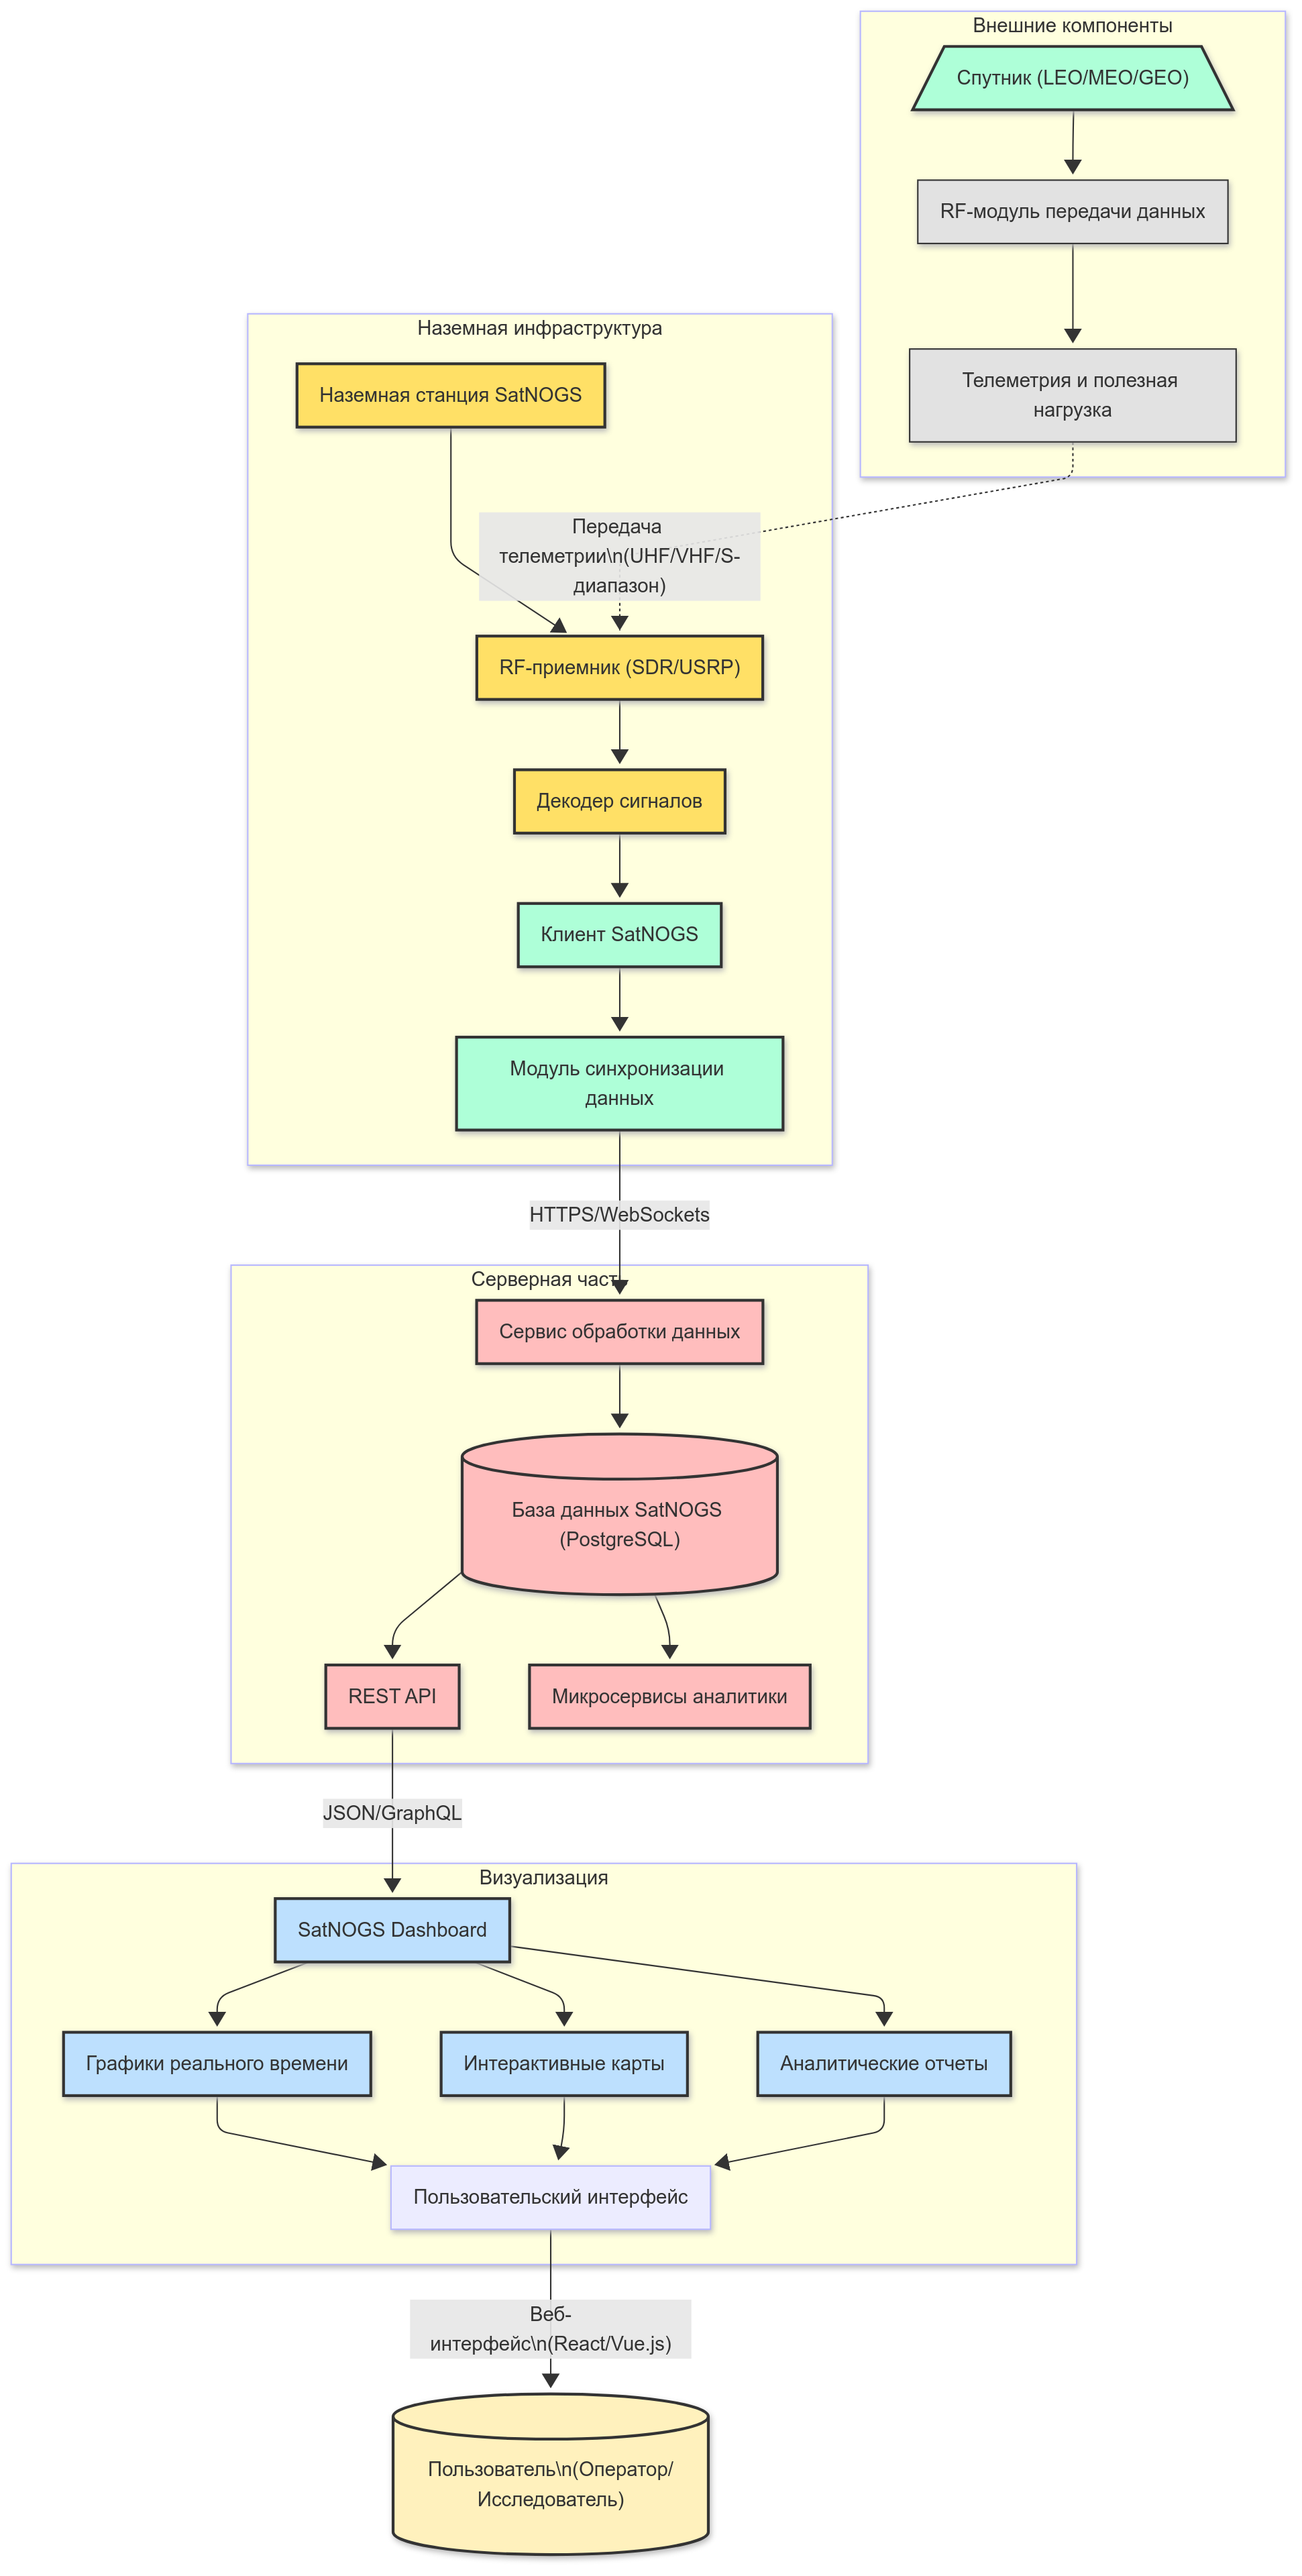
\includegraphics[width=0.7\textwidth]{satnogs_data_flow}
	\caption{Поток данных SatNOGS в Dashboard endpoint}
	\label{fig:satnogs_data_flow}
\end{figure}

\section{SatNOGS Dashboard}

SatNOGS Dashboard представляет собой ключевой компонент в нашей
исследовательской работе, выступая в качестве основного источника данных для
обучения моделей. После детального анализа архитектуры системы было определено
оптимальное место для извлечения данных. Dashboard Grafana в рамках экосистемы
SatNOGS предоставляет уже предобработанные данные, прошедшие фильтрацию и
дедупликацию посредством построения временных рядов. Несмотря на то, что
система содержит информацию только о приблизительно 120 спутниках, этот объем
является достаточным для анализа критических метрик и позволяет существенно
сократить затраты времени и вычислительных ресурсов на обучение, при этом
обеспечивая независимость от инфраструктуры SatNOGS.

Grafana -- это мощная платформа для визуализации и анализа данных, которая
позволяет создавать интерактивные дашборды на основе различных источников
данных \cite{grafana_docs}. Пример такого дашборда можно увидеть на рисунке
\ref{fig:grafana_example}.
Grafana широко используется для мониторинга систем и приложений, предоставляя
пользователям возможность отслеживать ключевые метрики в реальном времени.

\begin{figure}[H]
	\centering
	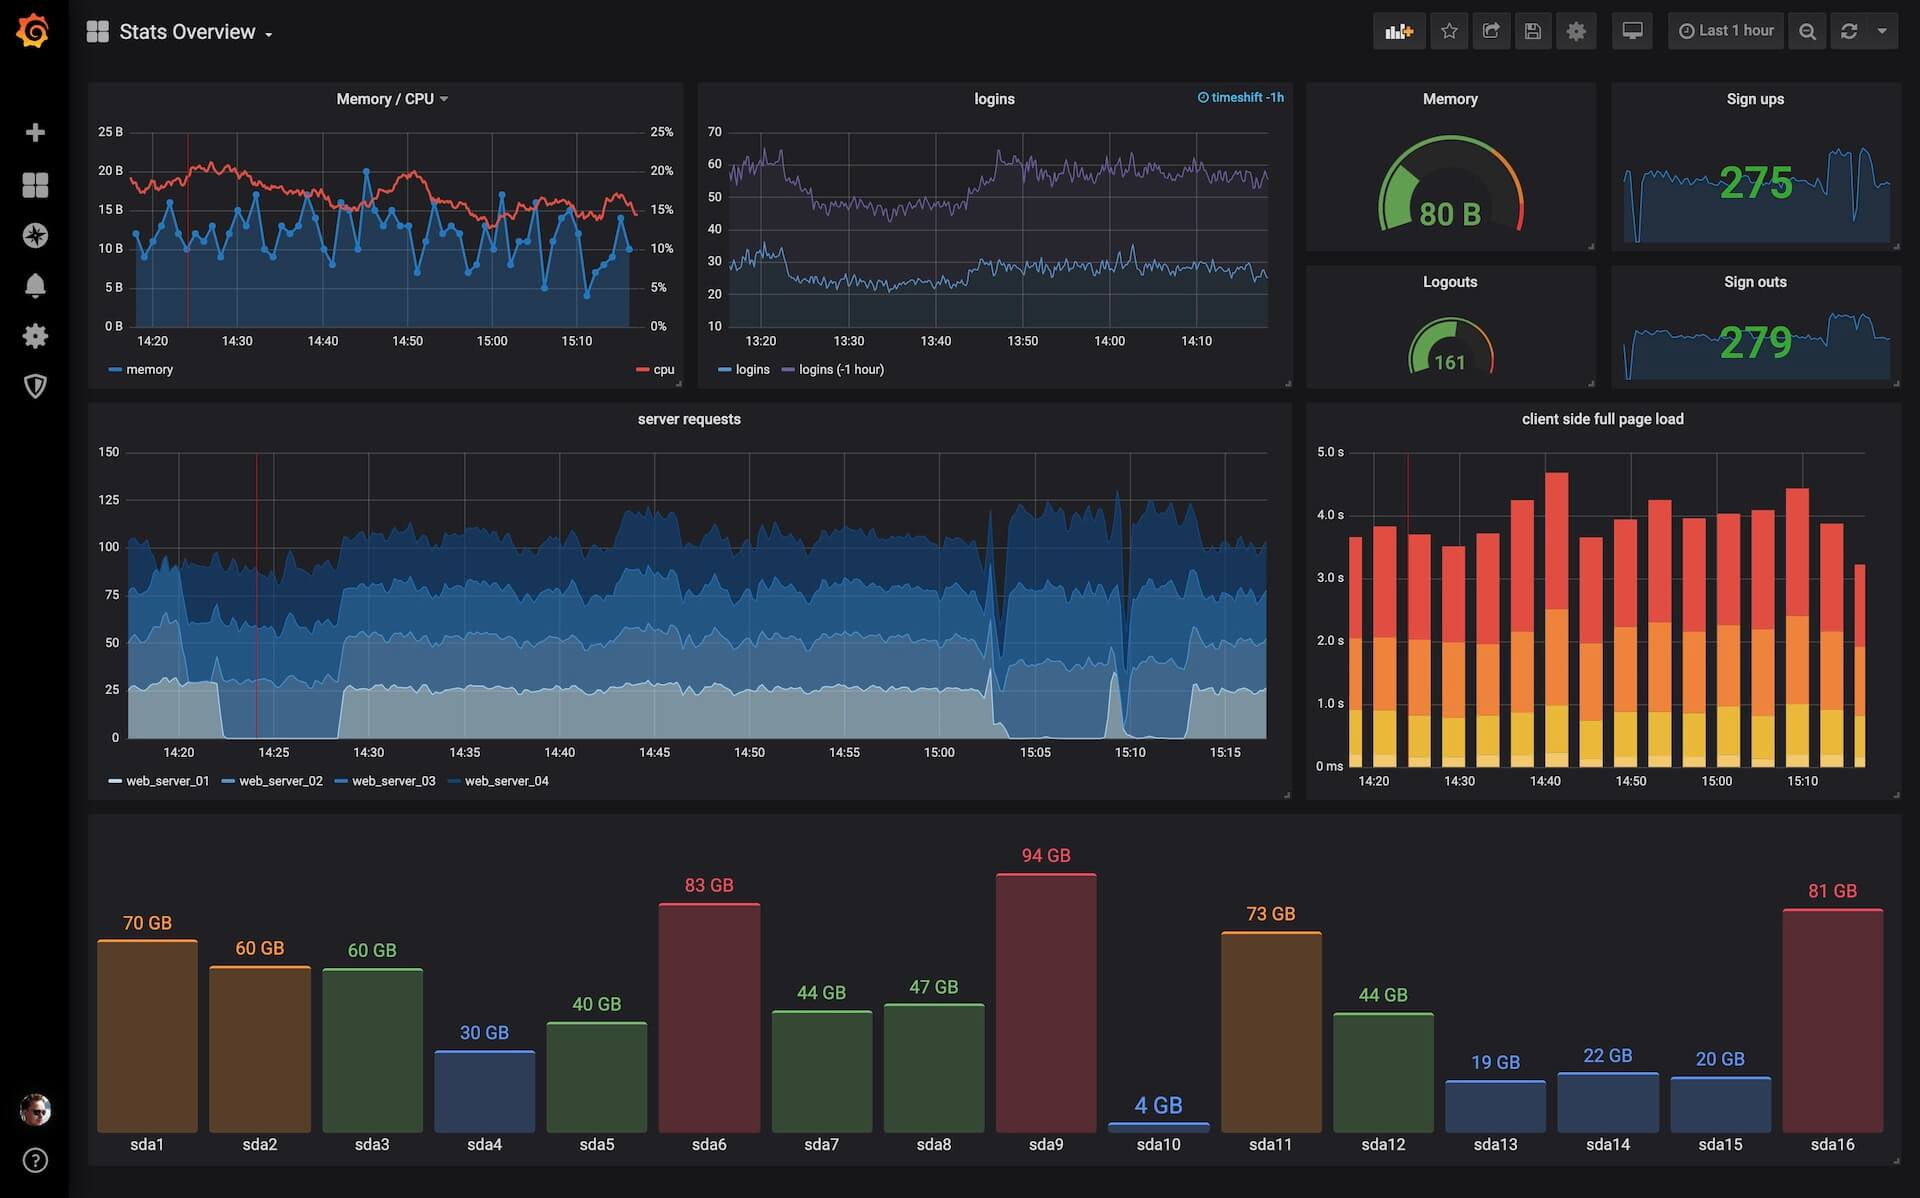
\includegraphics[width=1.0\textwidth]{grafana_example}
	\caption{Пример страницы с данными в Grafana Enterprise}
	\label{fig:grafana_example}
\end{figure}

В контексте SatNOGS Dashboard, Grafana работает с базой данных
\textbf{InfluxDB} \cite{influxdb_docs}, которая предназначена для хранения
временных рядов данных, таких как телеметрия спутников. Данные поступают от
наземных станций, обрабатываются клиентом SatNOGS и сохраняются в InfluxDB.
Затем Grafana использует API для доступа к этим данным и их визуализации на
дашбордах.

Однако стоит отметить, что доступ к API Grafana Dashboard SatNOGS был закрыт,
что ограничивает возможности пользователей в получении данных напрямую. Более
того, Grafana не предоставляет свои услуги пользователям из России и Беларуси в
связи с санциями \cite{grafana_community_post}, что создает дополнительные
сложности для разработчиков и исследователей из этих стран. Это делает Grafana
ненадежной платформой для работы в нашем регионе.

В ответ на эти ограничения нами разрабатывается специализированный парсер для
обхода существующих барьеров и получения необходимых данных. Данный инструмент
будет подробно рассмотрен в последующих разделах работы, поскольку он является
ключевым компонентом для интеграции данных из SatNOGS Dashboard в нашу систему
анализа и визуализации.

Таким образом, несмотря на значительный потенциал Grafana как инструмента
визуализации, текущие ограничения доступа существенно снижают её практическую
ценность для пользователей из определённых регионов, что обуславливает
необходимость разработки альтернативных методов работы с данными.
Схему работы SatNOGS Dashboard можно наблюдать на рисунке
\ref{fig:grafana_infra}.

\begin{figure}[H]
	\centering
	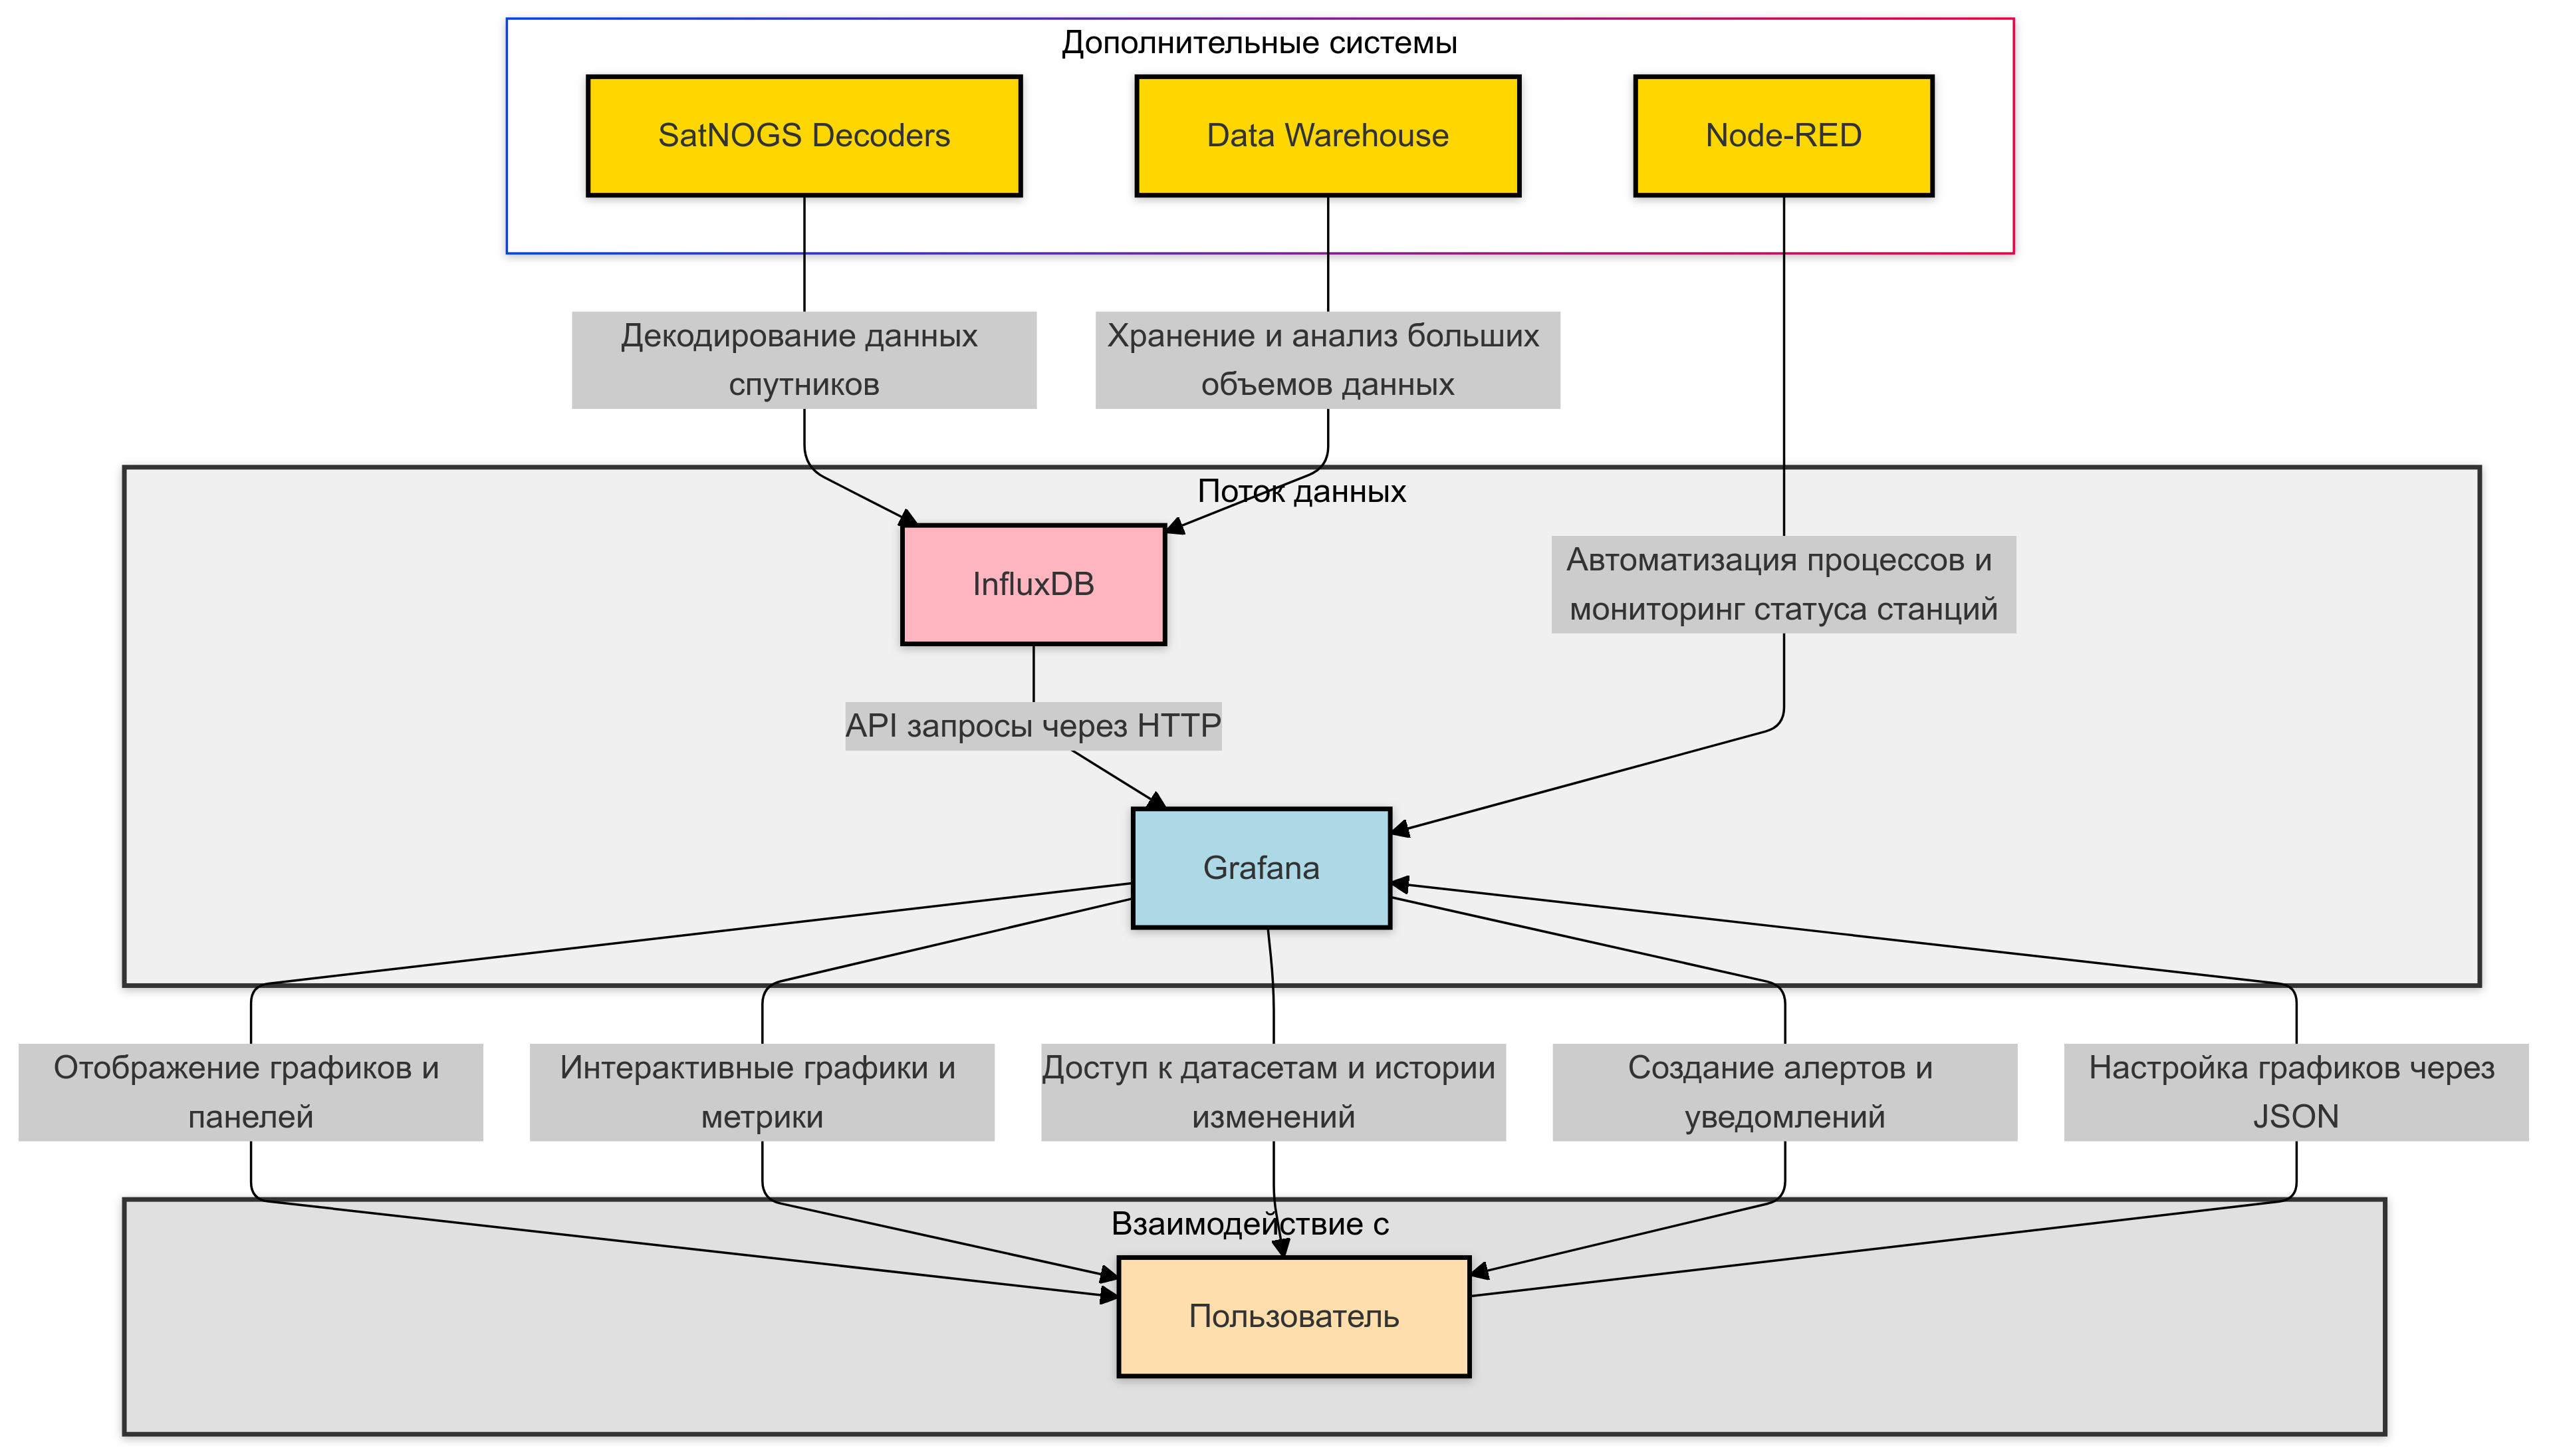
\includegraphics[width=1.0\textwidth]{grafana_infra}
	\caption{Подробное устройство SatNOGS Dashboard}
	\label{fig:grafana_infra}
\end{figure}


Разберем схему архитектуры фронтенд-части системы
\ref{fig:grafana_frontend_structure}
Grafana.
Данная схема иллюстрирует взаимодействие компонентов пользовательского
интерфейса Grafana и потоки данных между ними.

\subsection{Устройство frontend SatNOGS Dashboard}
\begin{figure}[htbp]
	\centering
	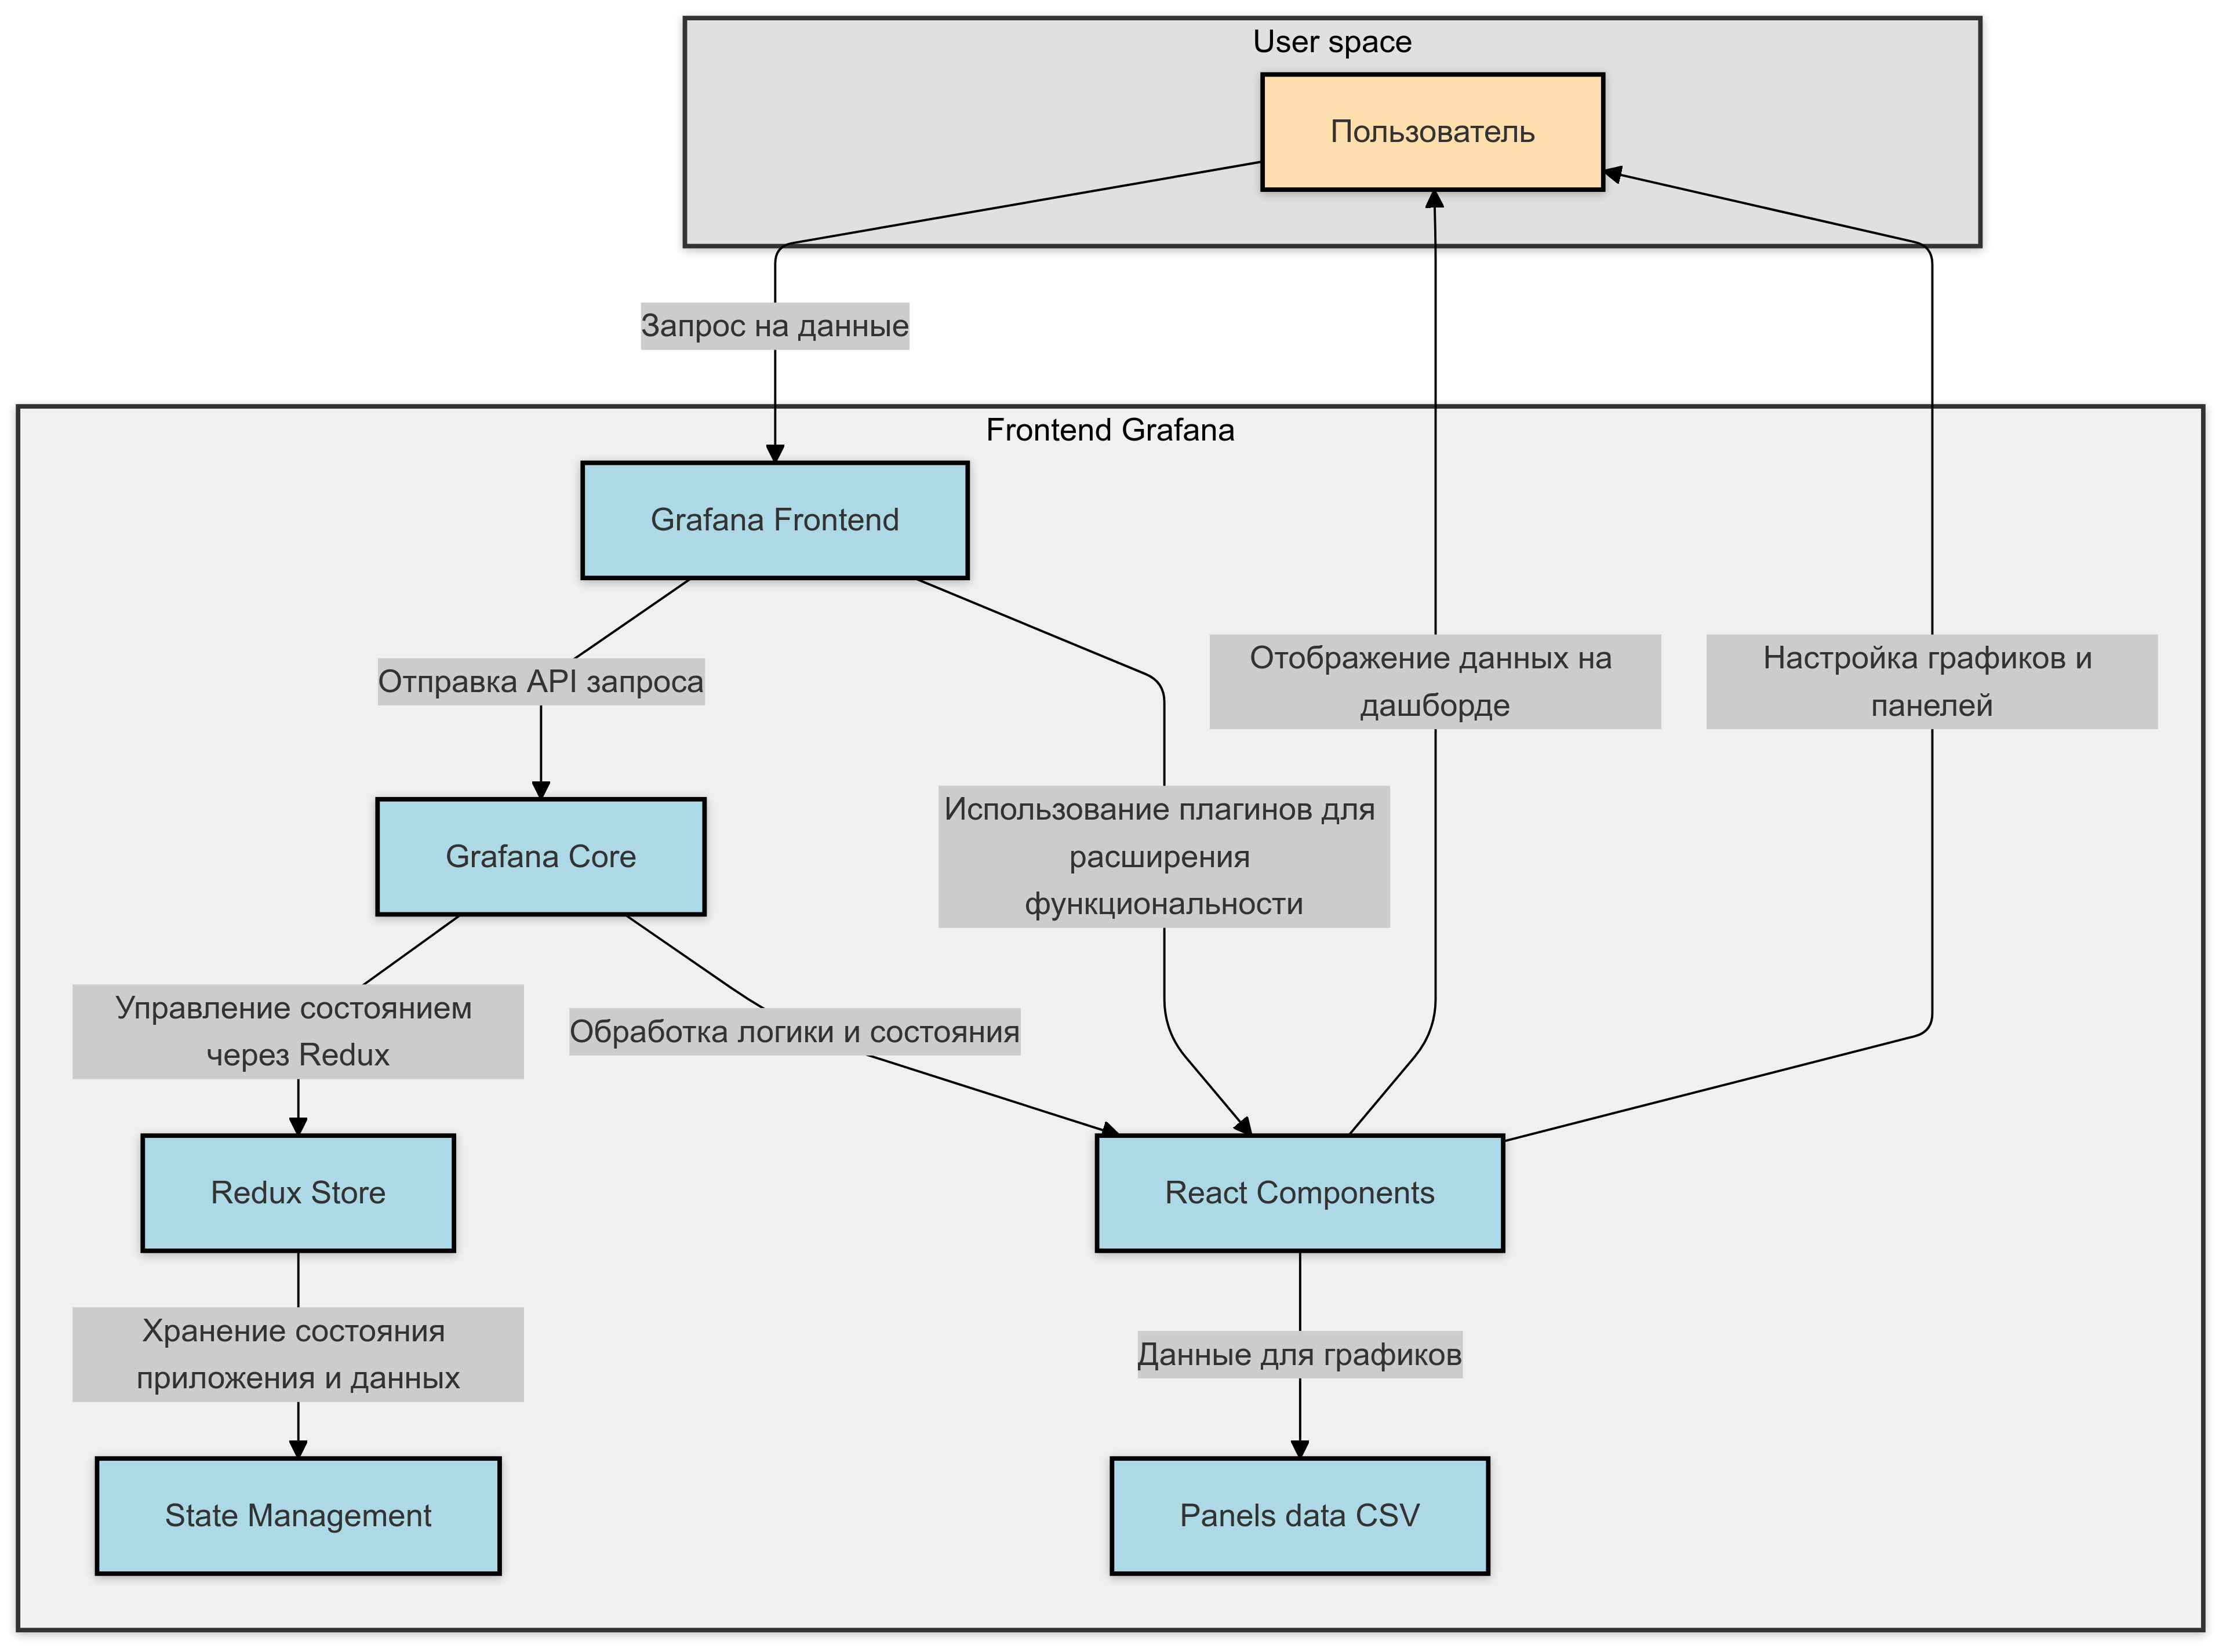
\includegraphics[width=1.0\textwidth]{grafana_frontend_structure}
	\caption{Построение frontend части grafana \cite{react_managing_state}}
	\label{fig:grafana_frontend_structure}
\end{figure}

Архитектура построена по многоуровневому принципу, где пользовательское
пространство (User space) взаимодействует с фронтенд-частью Grafana через
запросы на получение данных. Фронтенд Grafana состоит из нескольких ключевых
компонентов: Grafana Frontend, Grafana Core, Redux Store, State Management,
React Components и Panels data CSV.

Процесс работы системы начинается с запроса пользователя на получение данных,
который обрабатывается компонентом Grafana Frontend. Этот компонент отправляет
API-запросы к Grafana Core, который выполняет обработку логики и состояния.
Grafana Core взаимодействует с Redux Store для управления состоянием приложения
через механизм Redux. State Management отвечает за хранение состояния
приложения и данных.

React Components играют центральную роль в системе, обеспечивая отображение
данных на дашборде, настройку графиков и панелей, а также расширение
функциональности через плагины. Компонент Panels data CSV отвечает за
подготовку данных для графиков.

Для эффективного парсинга данной системы следует сосредоточиться на компоненте
Panels data CSV, который содержит структурированные данные для визуализации, а
также на API-запросах между Grafana Frontend и Grafana Core. Стратегия парсинга
должна учитывать, что данные проходят через несколько уровней обработки,
включая React Components, и хранятся в Redux Store. Понимание этой архитектуры
позволяет определить оптимальные точки извлечения данных и методы обхода
возможных ограничений доступа к API.

\section{Веб скраппер данных}

Представленный скрипт реализует асинхронный механизм извлечения данных из
панелей Grafana Dashboard с использованием библиотеки Playwright для
автоматизации браузера. Рассмотрим его архитектуру и принципы работы в деталях.

\subsection{Архитектура и основные компоненты}

Скрипт построен на основе асинхронной модели программирования Python с
использованием библиотеки asyncio, представляющей собой стандартный
инструментарий для реализации конкурентного выполнения кода. Данная библиотека,
введенная в Python 3.4 и дополненная синтаксисом async/await в Python 3.5,
обеспечивает эффективную обработку множества HTTP-запросов параллельно без
блокировки основной программы.

Архитектура скрипта характеризуется четким разделением основной логики на
функциональные блоки, образующие целостную систему извлечения данных. Блок
управления выполнением осуществляет настройку пулов потоков, дифференцируя
операции ввода-вывода и вычислительные процессы для оптимального использования
системных ресурсов. Механизмы формирования трафика реализуют регулирование
интенсивности запросов, предотвращая возможные блокировки со стороны сервера при
чрезмерной нагрузке.

Существенную роль в функционировании скрипта играет блок разрешения путей,
определяющий расположение JavaScript-файлов, необходимых для взаимодействия с
интерфейсом Grafana. Блок валидации данных обеспечивает проверку и фильтрацию
извлекаемой информации, гарантируя ее соответствие заданным критериям качества.
Завершающим звеном в цепи обработки является блок обработки измерений,
выполняющий анализ и нормализацию единиц измерения в полученных данных.

Центральным элементом всей системы выступает функция grafana\_fetch, которая
инициирует процесс извлечения данных. Данная функция запускает браузер Chromium
посредством библиотеки Playwright и координирует работу всех вышеописанных
компонентов, обеспечивая их согласованное функционирование в рамках единого
цикла событий. Благодаря использованию асинхронного подхода, скрипт способен
эффективно управлять множеством одновременно выполняющихся задач без
существенных затрат ресурсов, что особенно важно при обработке большого
количества HTTP-запросов.

\subsection{Технические особенности реализации}

Скрипт использует ряд технических приемов для повышения эффективности и
надежности, представляющих собой комплексное решение задачи оптимизации
извлечения данных. Асинхронное программирование, реализованное посредством
библиотеки asyncio, обеспечивает эффективную обработку множества запросов
параллельно, что позволяет максимизировать пропускную способность системы при
минимальном использовании вычислительных ресурсов. Данный подход особенно
эффективен при работе с сетевыми операциями, характеризующимися значительными
задержками.

Важным архитектурным решением является разделение операций на IO-bound
(ввод-вывод) и CPU-bound (вычисления) с использованием отдельных пулов потоков.
Такая дифференциация позволяет оптимизировать использование ресурсов системы,
предотвращая блокировку основного потока выполнения при выполнении длительных
операций ввода-вывода и обеспечивая эффективное распределение вычислительной
нагрузки между доступными ядрами процессора.

Механизм регулирования трафика реализован посредством применения случайных
задержек (jitter) между запросами и обработки панелей пакетами с паузами между
ними. Данный подход существенно снижает риск блокировки со стороны сервера,
который может интерпретировать большое количество одновременных запросов как
потенциальную DoS-атаку. Введение стохастического элемента в процесс
формирования запросов делает их паттерн более приближенным к естественному
поведению пользователя.

Комплексная система обработки исключений представляет собой многоуровневый
механизм, обеспечивающий устойчивость скрипта к сбоям отдельных компонентов.
Данная система позволяет продолжать работу даже при возникновении частичных
ошибок, изолируя проблемные участки и предотвращая каскадное распространение
сбоев на весь процесс извлечения данных.

Завершающим элементом оптимизации является применение параллельной обработки
данных с использованием библиотеки pandas. Данный инструментарий обеспечивает
эффективную обработку и трансформацию данных посредством векторизованных
операций, что существенно повышает производительность при работе с большими
объемами информации по сравнению с традиционными итеративными подходами.

\subsection{Практическое применение}

Скрипт предоставляет мощный инструмент для автоматизированного извлечения
данных из Grafana Dashboard, что особенно ценно в контексте ограниченного
доступа к API или при наличии региональных ограничений. Он может быть
интегрирован в более широкие системы анализа данных или мониторинга,
обеспечивая независимость от инфраструктуры Grafana.

Основное преимущество данного подхода заключается в его способности обходить
ограничения стандартного API путем эмуляции взаимодействия пользователя с
интерфейсом. Это позволяет получать данные даже в случаях, когда прямой
доступ к API ограничен или недоступен.

\begin{figure}[H]
	\centering
	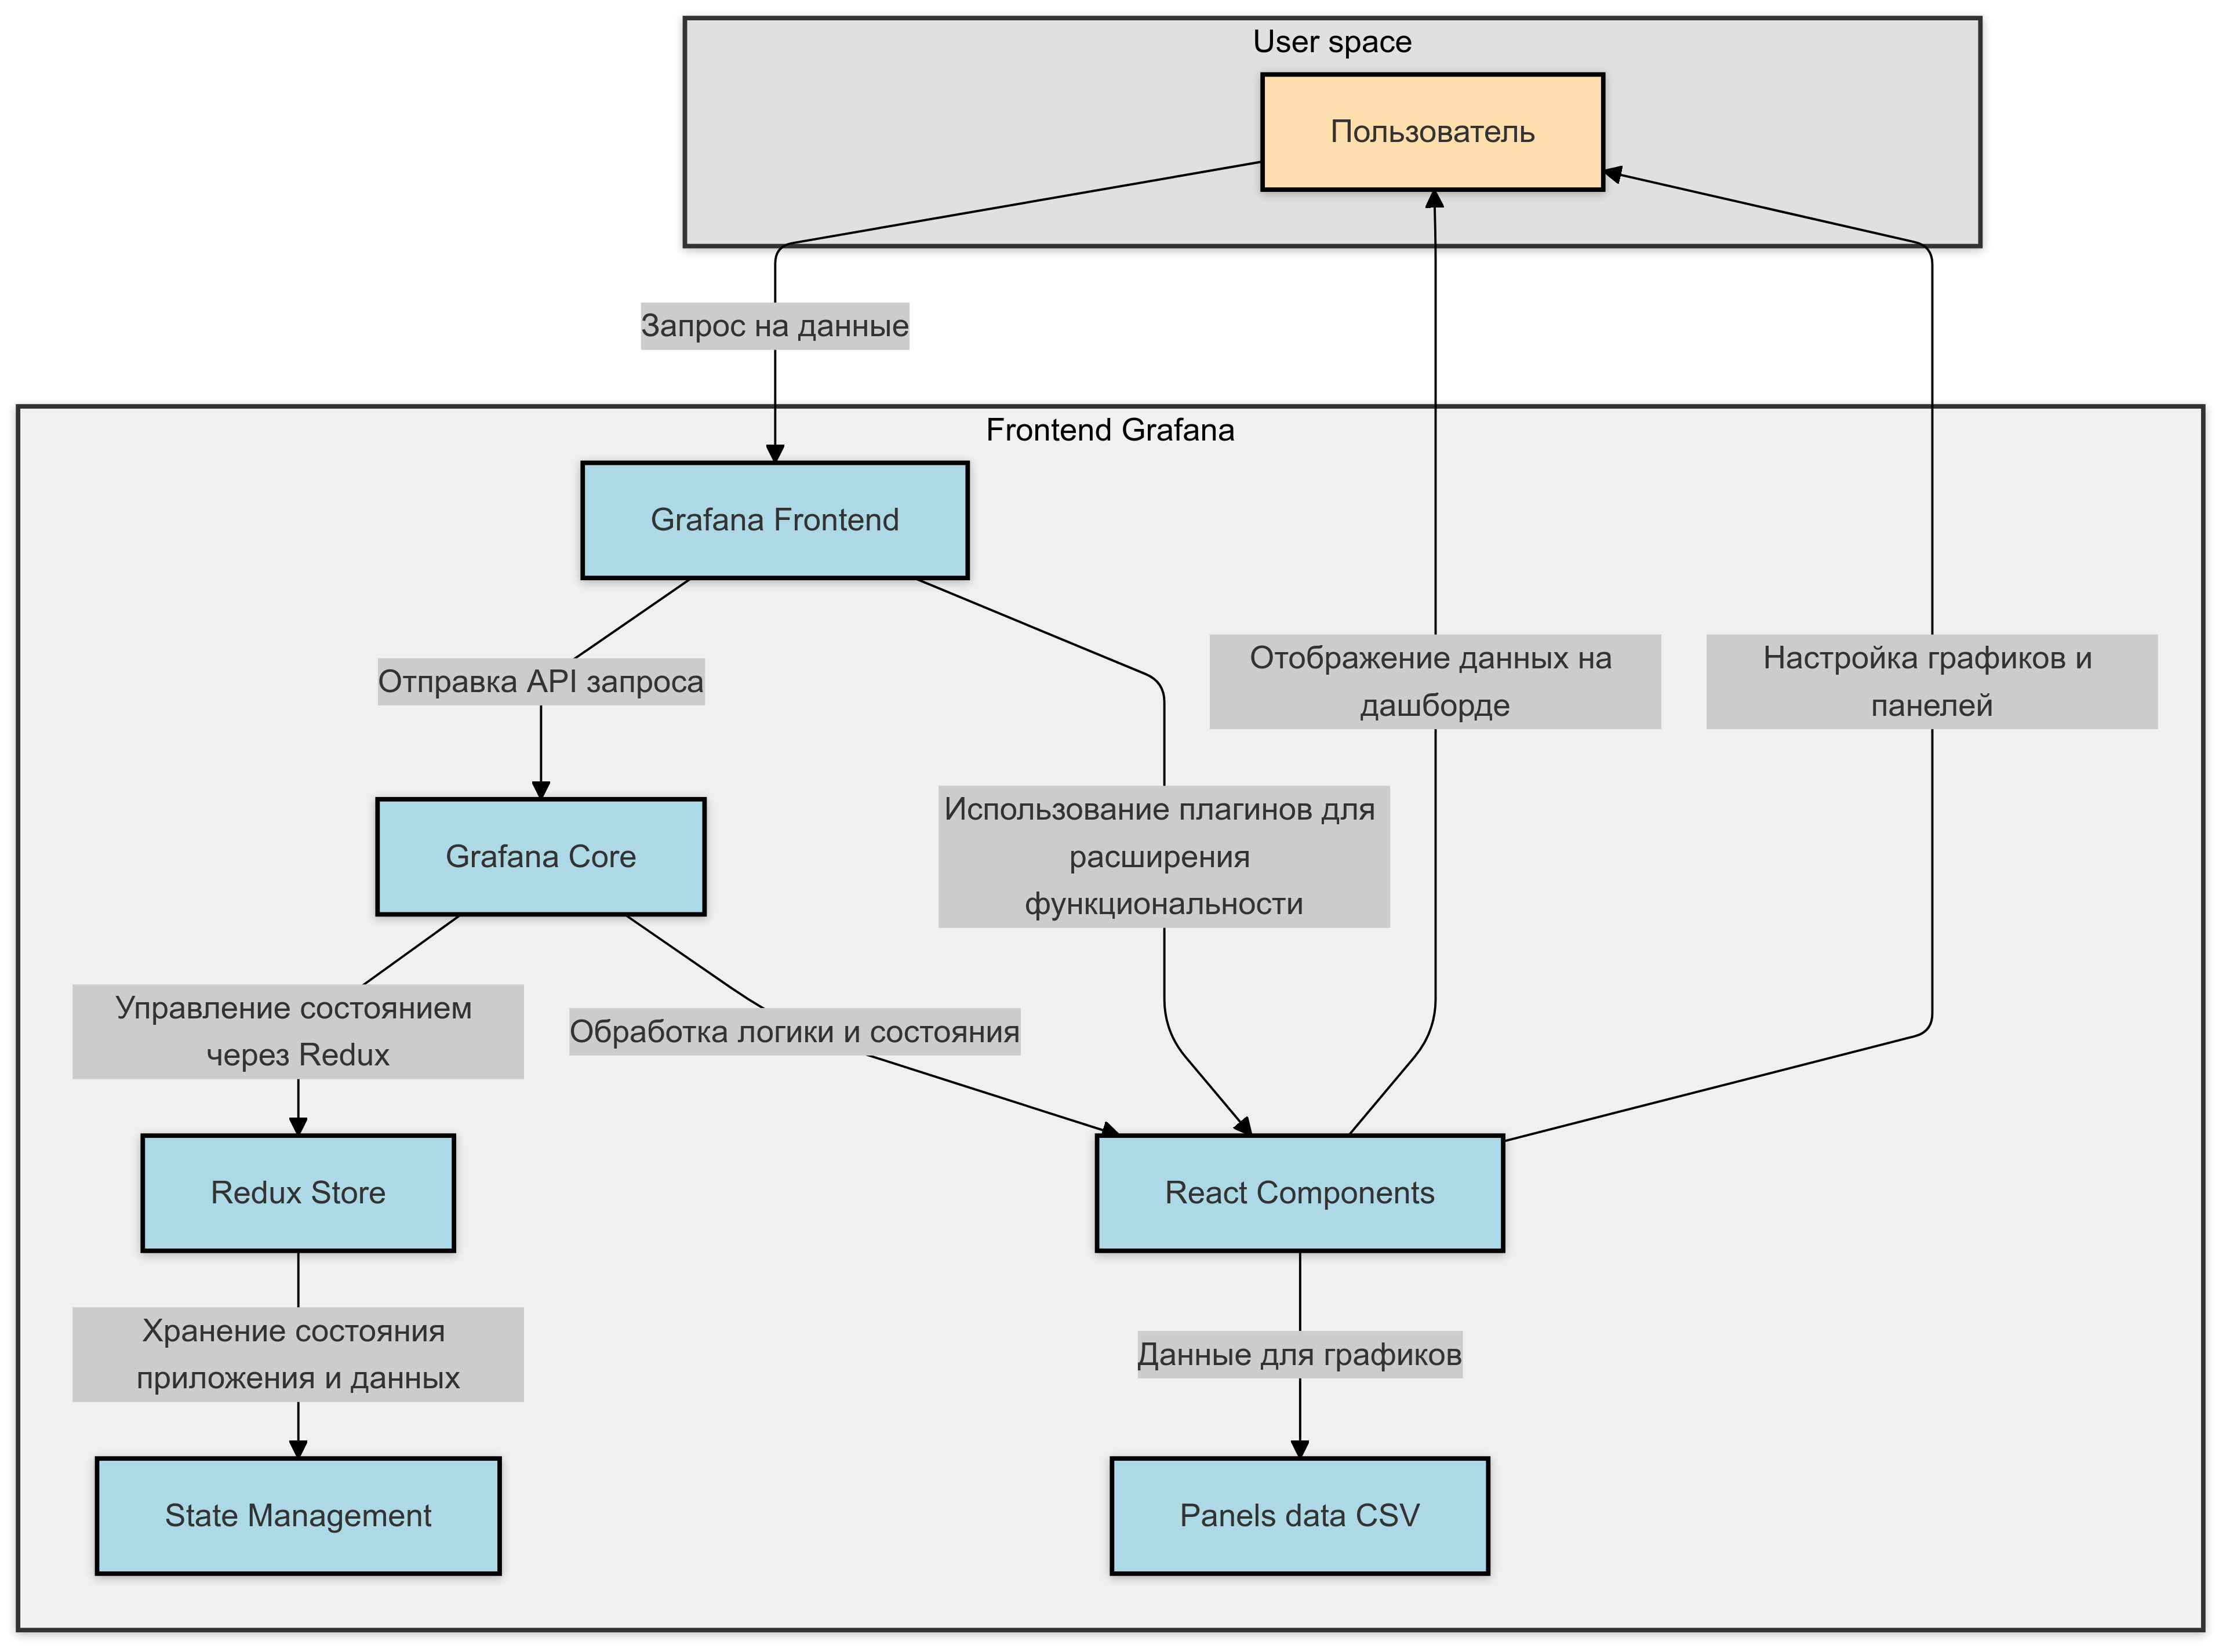
\includegraphics[width=0.9\textwidth]{grafana_frontend_structure}
	\caption{Структура фронтенд-части Grafana, иллюстрирующая компоненты, с которыми взаимодействует скрипт}
	\label{fig:grafana_frontend_structure_advanced}
\end{figure}

Как показано на рисунке \ref{fig:grafana_frontend_structure_advanced}, скрипт
взаимодействует с различными уровнями архитектуры Grafana, включая React
Components и Panels data CSV, что позволяет эффективно извлекать данные, минуя
стандартные ограничения API.

В контексте работы с SatNOGS Dashboard данный скрипт представляет собой
ключевой инструмент для получения телеметрических данных спутников, необходимых
для дальнейшего анализа и обучения моделей. Его применение позволяет преодолеть
ограничения доступа к данным и обеспечить независимость исследовательской
работы от внешней инфраструктуры.

\section{Выводы по главе}

В данной главе проанализирована экосистема SatNOGS как глобальная открытая платформа мониторинга спутников и определен SatNOGS Dashboard на базе Grafana/InfluxDB в качестве оптимального источника предобработанной телеметрии. Вследствие региональных ограничений API разработан асинхронный веб-скраппер с Playwright, обеспечивающий извлечение данных через эмуляцию пользовательского взаимодействия с регулированием трафика и параллельной обработкой. Реализованное решение создает независимую от внешней инфраструктуры систему сбора спутниковых данных для последующего анализа и обучения предиктивных моделей.
